\PassOptionsToPackage{unicode}{hyperref}
\PassOptionsToPackage{hyphens}{url}
\documentclass{article}
\setcounter{secnumdepth}{3}

\usepackage{amsmath,amssymb}
\usepackage{lmodern}
\usepackage{iftex}
\usepackage[letterpaper, margin=1in, top=0.5in, bottom=1in]{geometry}
\usepackage{listings}
\usepackage{color}
\usepackage{titling}
\usepackage{graphicx}
\usepackage{hyperref}

\ifPDFTeX
  \usepackage[T1]{fontenc}
  \usepackage[utf8]{inputenc}
  \usepackage{textcomp} 
\else 
  \usepackage{unicode-math}
  \defaultfontfeatures{Scale=MatchLowercase}
  \defaultfontfeatures[\rmfamily]{Ligatures=TeX,Scale=1}
\fi
\IfFileExists{upquote.sty}{\usepackage{upquote}}{}
\IfFileExists{microtype.sty}{
  \usepackage[]{microtype}
  \UseMicrotypeSet[protrusion]{basicmath} 
}{}
\makeatletter
\@ifundefined{KOMAClassName}{
  \IfFileExists{parskip.sty}{
    \usepackage{parskip}
  }{
    \setlength{\parindent}{0pt}
    \setlength{\parskip}{6pt plus 2pt 2pt}}
}{
  \KOMAoptions{parskip=half}}
\makeatother
\usepackage{xcolor}
\usepackage{graphicx}

\makeatletter
\def\maxwidth{\ifdim\Gin@nat@width>\linewidth\linewidth\else\Gin@nat@width\fi}
\def\maxheight{\ifdim\Gin@nat@height>\textheight\textheight\else\Gin@nat@height\fi}
\makeatother
\setkeys{Gin}{width=\maxwidth,height=\maxheight,keepaspectratio}
\makeatletter
\def\fps@figure{htbp}
\makeatother
\setlength{\emergencystretch}{3em} 
\providecommand{\tightlist}{
  \setlength{\itemsep}{0pt}\setlength{\parskip}{0pt}}

\ifLuaTeX
  \usepackage{selnolig}  
\fi
\IfFileExists{bookmark.sty}{\usepackage{bookmark}}{\usepackage{hyperref}}
\IfFileExists{xurl.sty}{\usepackage{xurl}}{} 
\urlstyle{same}
\hypersetup{
  hidelinks,
  pdfcreator={LaTeX via pandoc}}

\title{Artifacts - Sprint 3}
\date{}

\begin{document}

\maketitle

\hypertarget{sos-s3} {
\section{Scrum of Scrums}\label{Scrum of Scrums} 
At this point, the team had reorginazed the Epics due to the new architecture 
changes. Having Screen, Bridge and Games as main Epics.
During this sprint, while working on User Story #87, there was a refactoring 
in the architecture due to GUI should be running along with the game. 
Then, in the Lead's Daily a discussion occurred about that change, having it 
as an agreement furthermore, the contract (frontend-library) been terminated in its initial version.
}

\href{https://github.com/Pending-Name-21/arquitecture/pull/12}{Link: GUI Refactor - Pull Request on GitHub}.

\href{https://tree.taiga.io/project/joseluis-teran-coffeetime/taskboard/sprint-3-8974}{Link: User Stories of Sprint 3 on Taiga}.

\begin{figure}
\centering
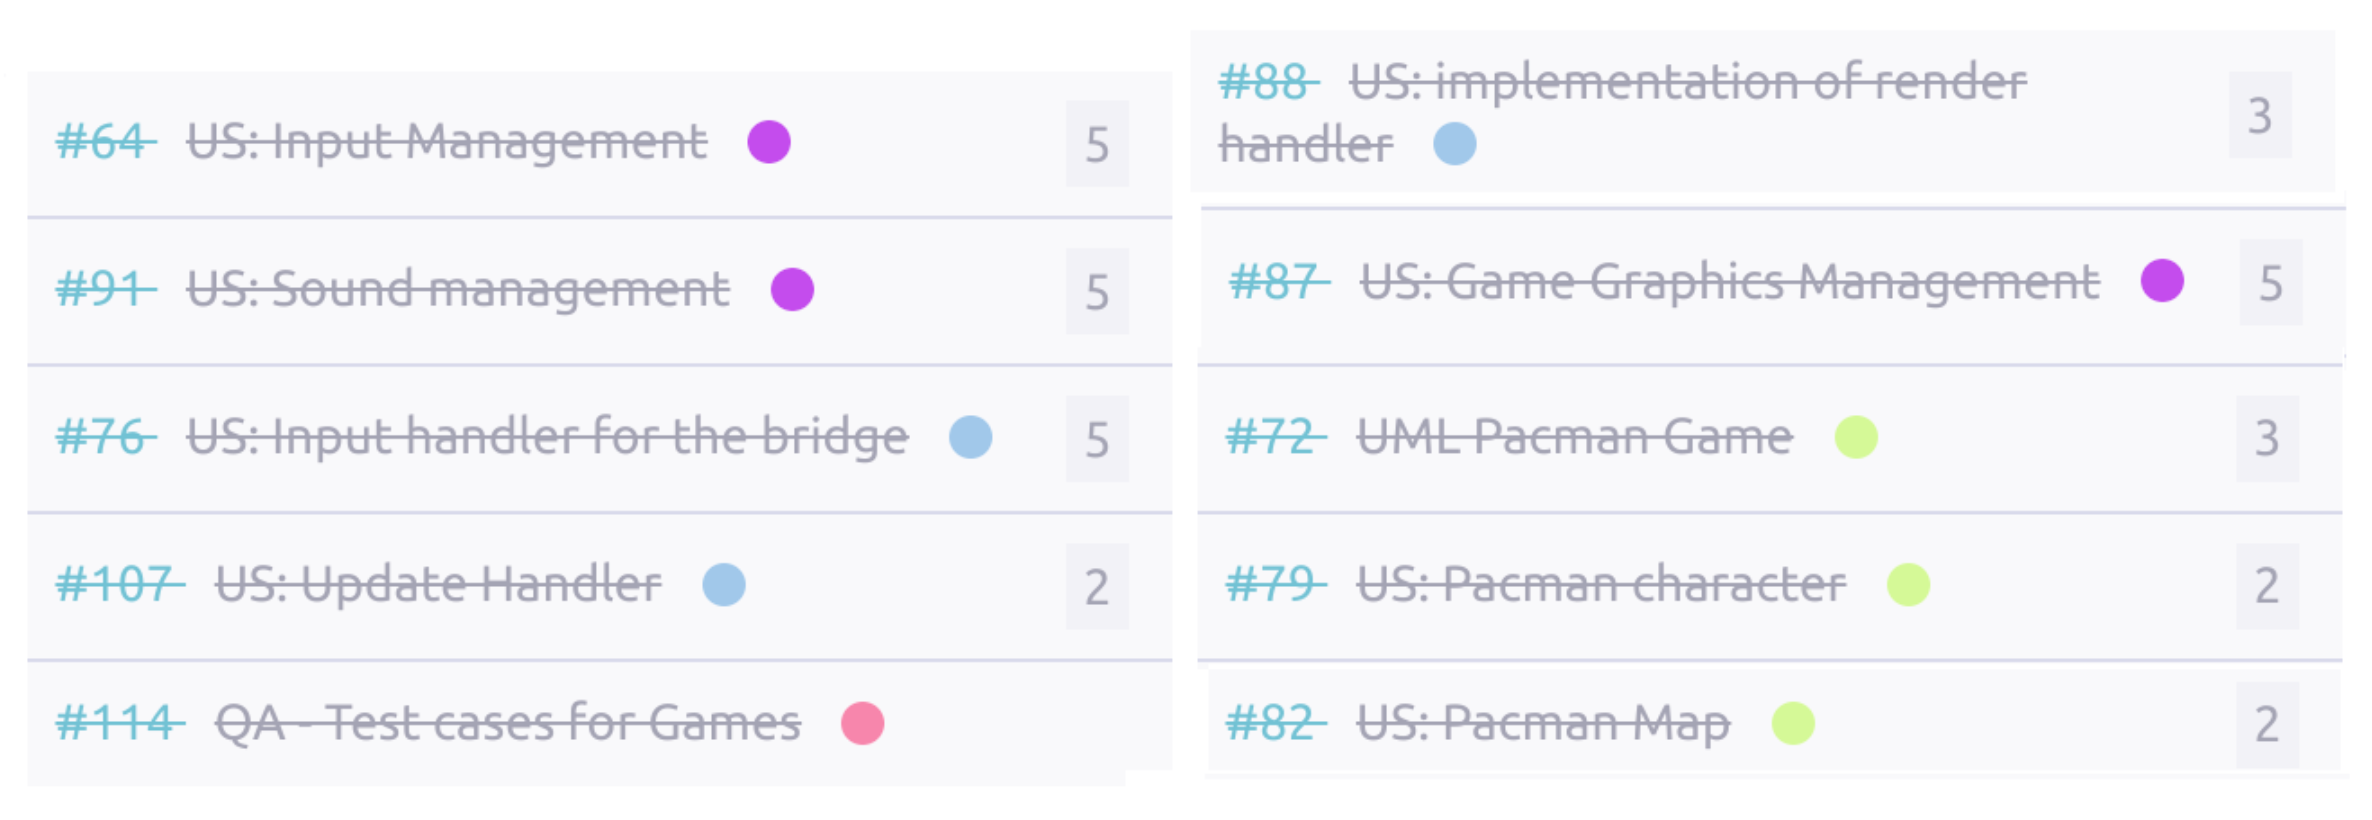
\includegraphics[width=16cm, height=10cm]{./assets/us-s3.png}
\end{figure}

\hypertarget{burndownchart-s3}{
\section{Burn Down Chart}\label{Burn Down Chart S3}}
\href{https://tree.taiga.io/project/joseluis-teran-coffeetime/taskboard/sprint-3-8974}{Link: Sprint 3 Board on Taiga}.

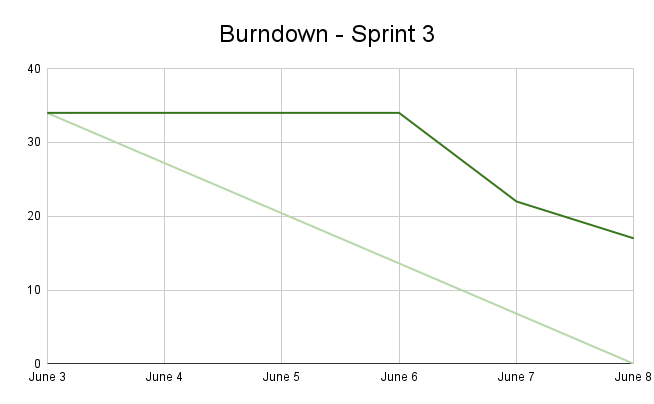
\includegraphics[width=\textwidth]{./assets/Burndown - Sprint 3.png}

\hypertarget{startstopcontinueactionitems-s3}{
\section{Start-Stop-Continue-Action Items}\label{Start-Stop-Continue-Action Items S2}}
\href{https://miro.com/app/board/uXjVKDO7l8M=/?moveToWidget=3458764590247889881&cot=14}{Link: Start-Stop-Continue-Action Items Sprint 3 on Miro}.

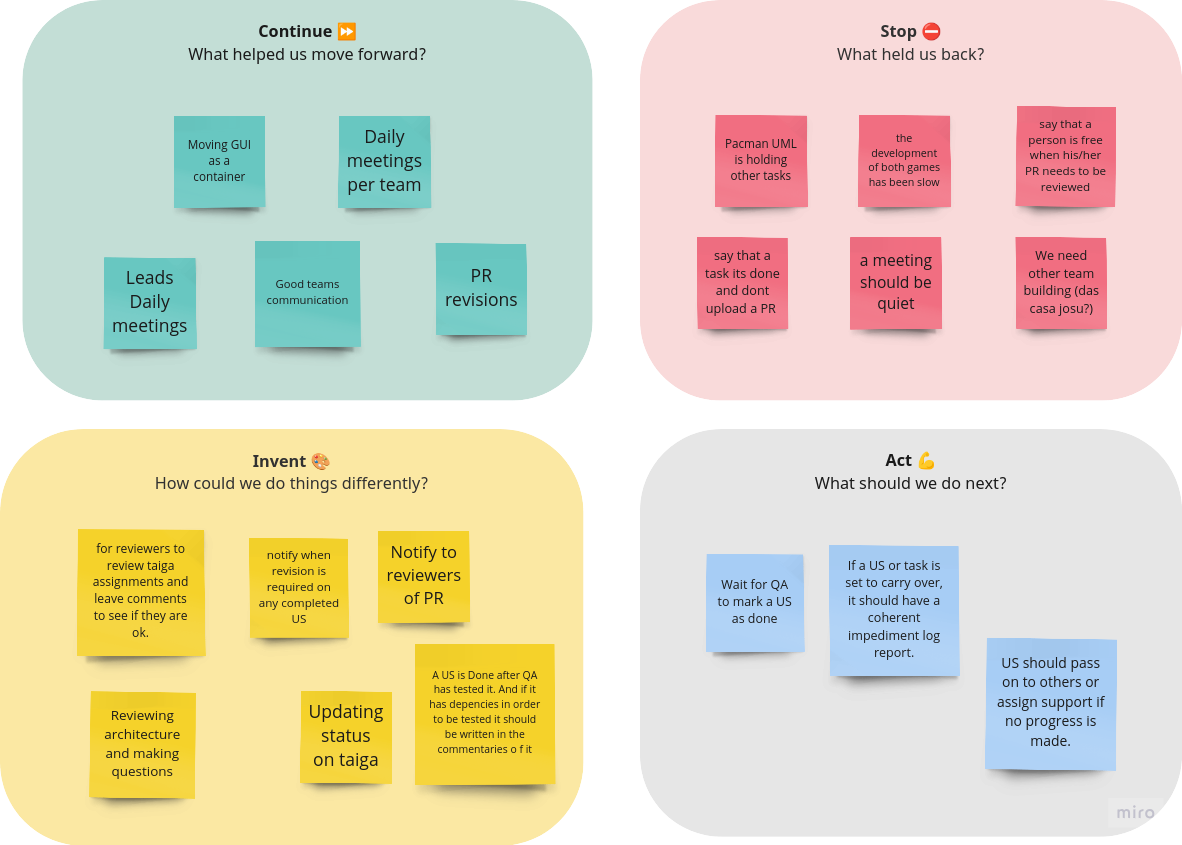
\includegraphics[width=\textwidth]{./assets/retrospective-s3.png}

\end{document}
